\documentclass[12pt, fullpage,letterpaper]{article}

\usepackage[margin=1in]{geometry}
\usepackage{url}
\usepackage{amsmath}
\usepackage{amssymb}
\usepackage{xspace}
\usepackage{graphicx}
\usepackage{hyperref}
\usepackage{listings}

\newcommand{\semester}{Spring 2019}
\newcommand{\assignmentId}{5}
\newcommand{\releaseDate}{9 Apr, 2019}
\newcommand{\dueDate}{11:59pm, 24 Apr, 2019}

\newcommand{\bx}{{\bf x}}
\newcommand{\bw}{{\bf w}}

\title{CS 5350/6350: Machine Learining \semester}
\author{Homework \assignmentId}
\date{Handed out: \releaseDate\\
	Due: \dueDate}


\title{CS 5350/6350: Machine Learning \semester}
\author{Homework \assignmentId}
\date{Handed out: \releaseDate\\
  Due date: \dueDate}

\begin{document}
\maketitle

% Math commands by Thomas Minka
\newcommand{\var}{{\rm var}}
\newcommand{\Tr}{^{\rm T}}
\newcommand{\vtrans}[2]{{#1}^{(#2)}}
\newcommand{\kron}{\otimes}
\newcommand{\schur}[2]{({#1} | {#2})}
\newcommand{\schurdet}[2]{\left| ({#1} | {#2}) \right|}
\newcommand{\had}{\circ}
\newcommand{\diag}{{\rm diag}}
\newcommand{\invdiag}{\diag^{-1}}
\newcommand{\rank}{{\rm rank}}
% careful: ``null'' is already a latex command
\newcommand{\nullsp}{{\rm null}}
\newcommand{\tr}{{\rm tr}}
\renewcommand{\vec}{{\rm vec}}
\newcommand{\vech}{{\rm vech}}
\renewcommand{\det}[1]{\left| #1 \right|}
\newcommand{\pdet}[1]{\left| #1 \right|_{+}}
\newcommand{\pinv}[1]{#1^{+}}
\newcommand{\erf}{{\rm erf}}
\newcommand{\hypergeom}[2]{{}_{#1}F_{#2}}

% boldface characters
\renewcommand{\a}{{\bf a}}
\renewcommand{\b}{{\bf b}}
\renewcommand{\c}{{\bf c}}
\renewcommand{\d}{{\rm d}}  % for derivatives
\newcommand{\e}{{\bf e}}
\newcommand{\f}{{\bf f}}
\newcommand{\g}{{\bf g}}
\newcommand{\h}{{\bf h}}
%\newcommand{\k}{{\bf k}}
% in Latex2e this must be renewcommand
\renewcommand{\k}{{\bf k}}
\newcommand{\m}{{\bf m}}
\newcommand{\mb}{{\bf m}}
\newcommand{\n}{{\bf n}}
\renewcommand{\o}{{\bf o}}
\newcommand{\p}{{\bf p}}
\newcommand{\q}{{\bf q}}
\renewcommand{\r}{{\bf r}}
\newcommand{\s}{{\bf s}}
\renewcommand{\t}{{\bf t}}
\renewcommand{\u}{{\bf u}}
\renewcommand{\v}{{\bf v}}
\newcommand{\w}{{\bf w}}
\newcommand{\x}{{\bf x}}
\newcommand{\y}{{\bf y}}
\newcommand{\z}{{\bf z}}
%s\newcommand{\l}{\boldsymbol{l}}
\newcommand{\A}{{\bf A}}
\newcommand{\B}{{\bf B}}
\newcommand{\C}{{\bf C}}
\newcommand{\D}{{\bf D}}
\newcommand{\E}{{\bf E}}
\newcommand{\F}{{\bf F}}
\newcommand{\G}{{\bf G}}
\renewcommand{\H}{{\bf H}}
\newcommand{\I}{{\bf I}}
\newcommand{\J}{{\bf J}}
\newcommand{\K}{{\bf K}}
\renewcommand{\L}{{\bf L}}
\newcommand{\M}{{\bf M}}
\newcommand{\N}{\mathcal{N}}  % for normal density
%\newcommand{\N}{{\bf N}}
\renewcommand{\O}{{\bf O}}
\renewcommand{\P}{{\bf P}}
\newcommand{\Q}{{\bf Q}}
\newcommand{\R}{{\bf R}}
\renewcommand{\S}{{\bf S}}
\newcommand{\T}{{\bf T}}
\newcommand{\U}{{\bf U}}
\newcommand{\V}{{\bf V}}
\newcommand{\W}{{\bf W}}
\newcommand{\X}{{\bf X}}
\newcommand{\Y}{{\bf Y}}
\newcommand{\Z}{{\bf Z}}

% this is for latex 2.09
% unfortunately, the result is slanted - use Latex2e instead
%\newcommand{\bfLambda}{\mbox{\boldmath$\Lambda$}}
% this is for Latex2e
\newcommand{\bfLambda}{\boldsymbol{\Lambda}}

% Yuan Qi's boldsymbol
\newcommand{\bsigma}{\boldsymbol{\sigma}}
\newcommand{\balpha}{\boldsymbol{\alpha}}
\newcommand{\bpsi}{\boldsymbol{\psi}}
\newcommand{\bphi}{\boldsymbol{\phi}}
\newcommand{\boldeta}{\boldsymbol{\eta}}
\newcommand{\Beta}{\boldsymbol{\eta}}
\newcommand{\btau}{\boldsymbol{\tau}}
\newcommand{\bvarphi}{\boldsymbol{\varphi}}
\newcommand{\bzeta}{\boldsymbol{\zeta}}

\newcommand{\blambda}{\boldsymbol{\lambda}}
\newcommand{\bLambda}{\mathbf{\Lambda}}
\newcommand{\bOmega}{\mathbf{\Omega}}
\newcommand{\bomega}{\mathbf{\omega}}
\newcommand{\bPi}{\mathbf{\Pi}}

\newcommand{\btheta}{\boldsymbol{\theta}}
\newcommand{\bpi}{\boldsymbol{\pi}}
\newcommand{\bxi}{\boldsymbol{\xi}}
\newcommand{\bSigma}{\boldsymbol{\Sigma}}

\newcommand{\bgamma}{\boldsymbol{\gamma}}
\newcommand{\bGamma}{\mathbf{\Gamma}}

\newcommand{\bmu}{\boldsymbol{\mu}}
\newcommand{\1}{{\bf 1}}
\newcommand{\0}{{\bf 0}}

% \newcommand{\comment}[1]{}

\newcommand{\bs}{\backslash}
\newcommand{\ben}{\begin{enumerate}}
\newcommand{\een}{\end{enumerate}}

 \newcommand{\notS}{{\backslash S}}
 \newcommand{\nots}{{\backslash s}}
 \newcommand{\noti}{{\backslash i}}
 \newcommand{\notj}{{\backslash j}}
 \newcommand{\nott}{\backslash t}
 \newcommand{\notone}{{\backslash 1}}
 \newcommand{\nottp}{\backslash t+1}
% \newcommand{\notz}{\backslash z}

\newcommand{\notk}{{^{\backslash k}}}
%\newcommand{\noti}{{^{\backslash i}}}
\newcommand{\notij}{{^{\backslash i,j}}}
\newcommand{\notg}{{^{\backslash g}}}
\newcommand{\wnoti}{{_{\w}^{\backslash i}}}
\newcommand{\wnotg}{{_{\w}^{\backslash g}}}
\newcommand{\vnotij}{{_{\v}^{\backslash i,j}}}
\newcommand{\vnotg}{{_{\v}^{\backslash g}}}
\newcommand{\half}{\frac{1}{2}}
\newcommand{\msgb}{m_{t \leftarrow t+1}}
\newcommand{\msgf}{m_{t \rightarrow t+1}}
\newcommand{\msgfp}{m_{t-1 \rightarrow t}}

\newcommand{\proj}[1]{{\rm proj}\negmedspace\left[#1\right]}
\newcommand{\argmin}{\operatornamewithlimits{argmin}}
\newcommand{\argmax}{\operatornamewithlimits{argmax}}

\newcommand{\dif}{\mathrm{d}}
\newcommand{\abs}[1]{\lvert#1\rvert}
\newcommand{\norm}[1]{\lVert#1\rVert}

%miscellaneous symbols
\newcommand{\ie}{{{i.e.,}}\xspace}
\newcommand{\eg}{{{\em e.g.,}}\xspace}
\newcommand{\EE}{\mathbb{E}}
\newcommand{\VV}{\mathbb{V}}
\newcommand{\sbr}[1]{\left[#1\right]}
\newcommand{\rbr}[1]{\left(#1\right)}
\newcommand{\cmt}[1]{}


\newcommand{\Hcal}{\mathcal{H}} 
{\footnotesize
	\begin{itemize}
		\item You are welcome to talk to other members of the class about
		the homework. I am more concerned that you understand the
		underlying concepts. However, you should write down your own
		solution. Please keep the class collaboration policy in mind.
		
		\item Feel free to discuss the homework with the instructor or the TAs.
		
		\item Your written solutions should be brief and clear. You do not need to include original problem descriptions in your solutions. You need to
		show your work, not just the final answer, but you do \emph{not}
		need to write it in gory detail. Your assignment should be {\bf no
			more than 15 pages}. Every extra page will cost a point.
		
		\item Handwritten solutions will not be accepted.
		
		
		\item {\em Your code should run on the CADE machines}. \textbf{You should
		include a shell script, {\tt run.sh}, that will execute your code
		in the CADE environment. Your code should produce similar output to what you include in your report.}
		
		You are responsible for ensuring that the grader can execute the
		code using only the included script. If you are using an
		esoteric programming language, you should make sure that its
		runtime is available on CADE.
		
		\item Please do not hand in binary files! We will {\em not} grade
		binary submissions.
		
		\item The homework is due by \textbf{midnight of the due date}. Please submit
		the homework on Canvas.
		
	\end{itemize}
}


\section{Paper Problems [40 points]}
\begin{enumerate}
	\item~[5 points] (Warm up) Suppose we have a composite function, $z = \sigma(y_1^2 +y_2y_3) $, where  $y_1 = 3x$, $y_2 = e^{-x}$, $y_3 = \mathrm{sin}(x)$, and $\sigma(\cdot)$ is the sigmoid activation function . Please use the chain rule to derive $\frac{\partial z}{\partial x}$ and  compute the derivative at $x=0$. 
	
	$\frac{\partial z}{\partial x} = \frac{\partial z}{\partial y_1}\frac{\partial y_1}{\partial x} + \frac{\partial z}{\partial y_2}\frac{\partial y_2}{\partial x} + \frac{\partial z}{\partial y_2}\frac{\partial y_2}{\partial x}$

	$ = (\frac{2e^{-x^2-yz}x}{\left(1+e^{-x^2-yz}\right)^2})(3) + (\frac{e^{-yz-x^2}z}{\left(1+e^{-x^2-yz}\right)^2})(-e^{-x}) + (\frac{e^{-yz-x^2}y}{\left(1+e^{-x^2-yz}\right)^2})(\mathrm{cos}(x))$
	
	$= \frac{6e^{-x^2-yz}x-e^{-x^2-x-yz}z+e^{-x^2-yz}y\cos \left(x\right)}{\left(e^{-x^2-yz}+1\right)^2}$
	
	
	
	\begin{figure*}
		\centering
		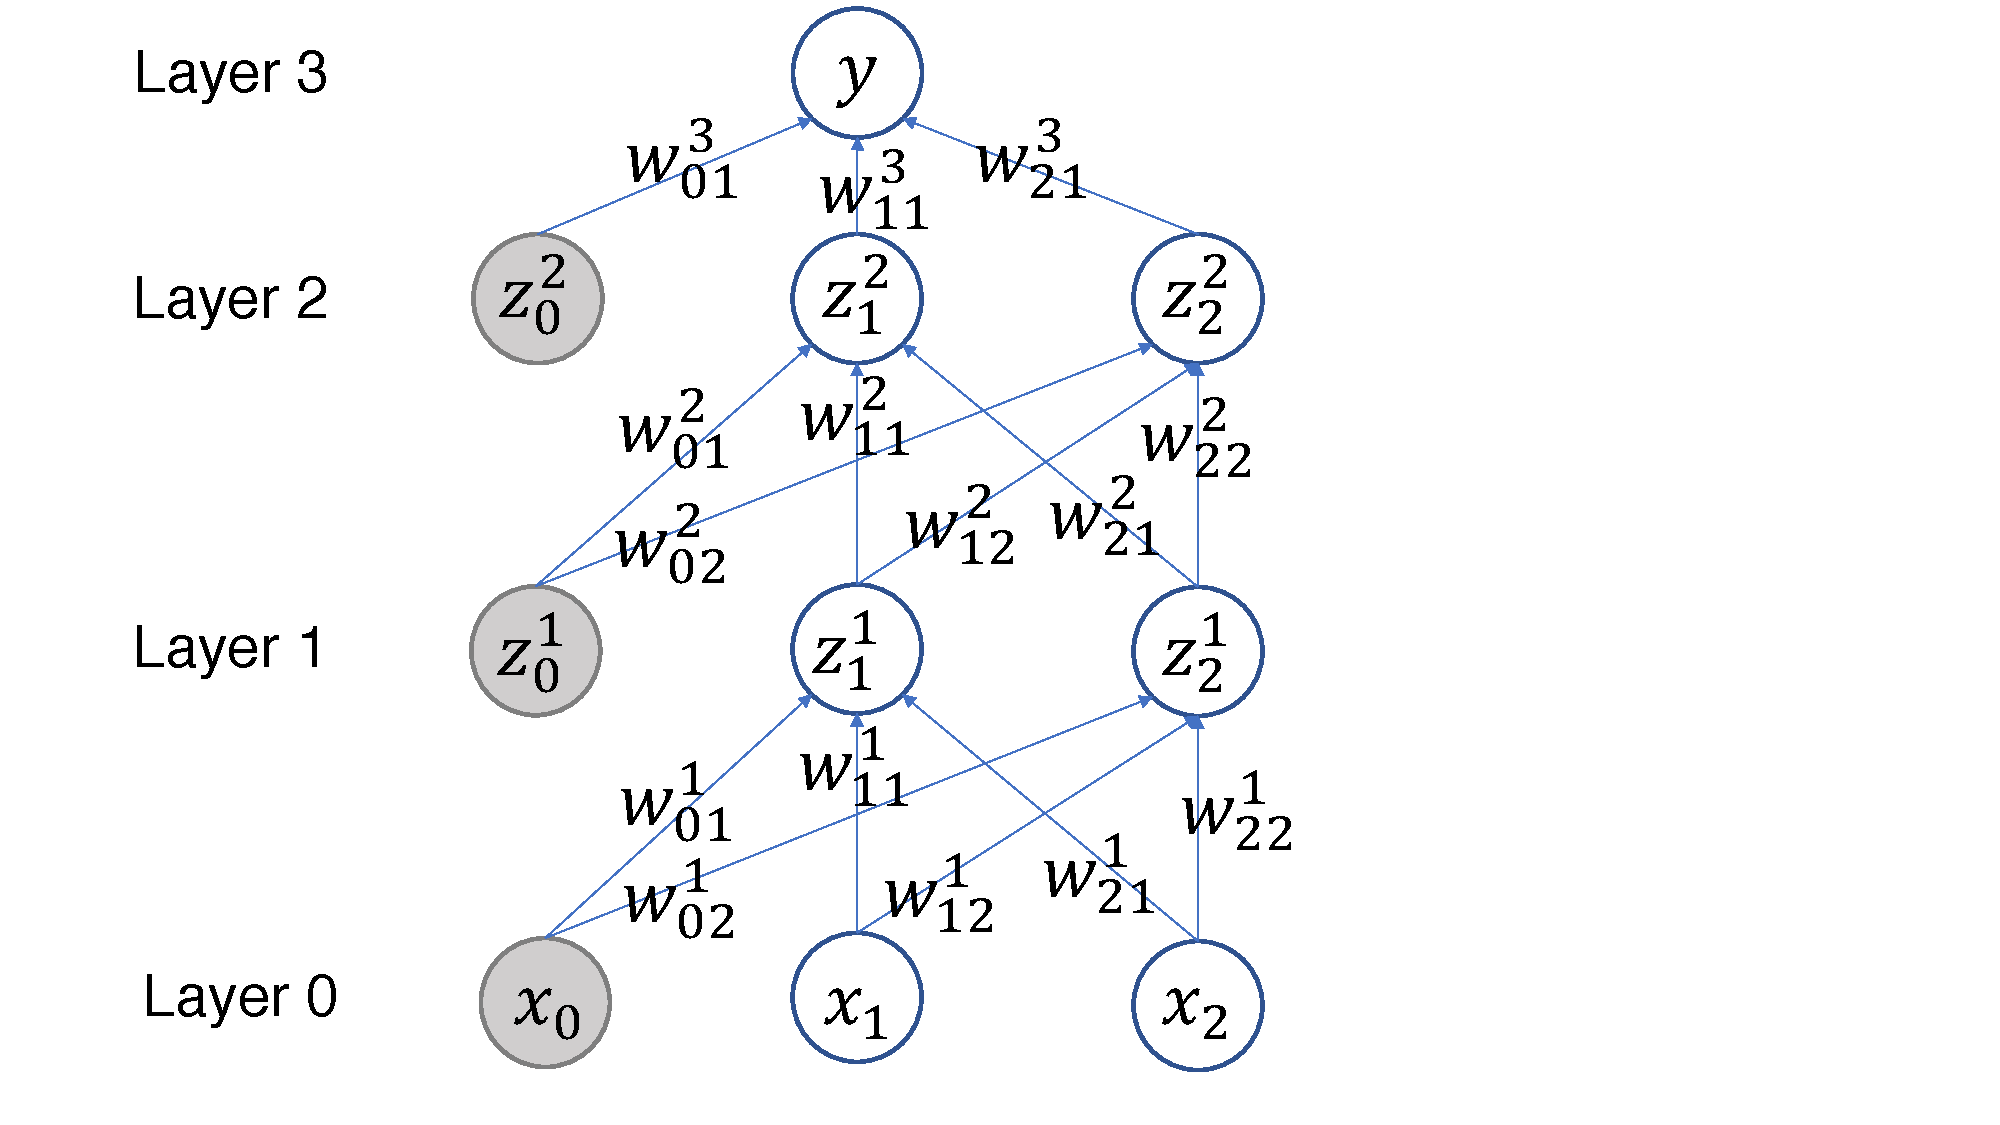
\includegraphics[width=1.0\textwidth]{fig.pdf}
		\caption{\small A three layer artificial neural network.} 
		\label{fig:3nn}
	\end{figure*}
	
	\begin{table}[h]
		\centering
		\begin{tabular}{c|cc}
			Layer & weigth  & value\\ 
			\hline\hline
			$1$ & $w_{01}^1$ & $-1$ \\ \hline
			$1$ & $w_{02}^1$ & $1$ \\ \hline
			$1$ & $w_{11}^1$ & $-2$ \\ \hline
			$1$ & $w_{12}^1$ & $2$ \\ \hline
			$1$ & $w_{21}^1$ & $-3$ \\ \hline
			$1$ & $w_{22}^1$ & $3$ \\ \hline
			$2$ & $w_{01}^2$ & $-1$ \\ \hline
			$2$ & $w_{02}^2$ & $1$ \\ \hline
			$2$ & $w_{11}^2$ & $-2$ \\ \hline
			$2$ & $w_{12}^2$ & $2$ \\ \hline
			$2$ & $w_{21}^2$ & $-3$ \\ \hline
			$2$ & $w_{22}^2$ & $3$ \\ \hline
			$3$ & $w_{01}^3$ & $-1$ \\ \hline
			$3$ & $w_{11}^3$ & $2$ \\ \hline
			$3$ & $w_{21}^3$ & $-1.5$ \\ \hline
		\end{tabular}
		\caption{Weight values.}
		\label{tb:w}
	\end{table}
	
	%forward pass
	\item~[5 points] Suppose we have a three-layered feed-forward neural network in hand. The architecture and the weights are defined in Figure \ref{fig:3nn}. We use the sigmoid activation function. Note that the shaded variables are the constant feature $1$, \ie $x_0 = z_{0}^1 = z_{0}^2 = 1$. As we discussed in the class, they are used to account for the bias parameters. 
	We have the values of all the edge weights in Table \ref{tb:w}. Now, given a new input example $\x=[1, 1, 1]$. Please use the forward pass to compute the output $y$. Please list every step in your computation, namely, how you calculate the variable value in each hidden unit, and how  you combine the variables in one layer to compute each variable in the next layer. Please be aware of the subtle difference in computing the variable value in the last layer (we emphasized it in the class). 
	
	%back-propgation
	
	$z^1_1 = \sigma(w^1_{01} + w^1_{11}x_1 + w^1_{21}x_2) = \sigma(-1 + -2*1 + -3*1) = \frac{1}{1+e^6} = 0.00247$
	
	$z^1_2 = \sigma(w^1_{02} + w^1_{12}x_1 + w^1_{22}x_2) = 0.99753$
	
	$z^2_1 = \sigma(w^2_{01} + w^2_{11}z^1_1 + w^2_{21}z^1_2) = 0.01803$
	
	$z^2_2 = \sigma(w^2_{02} + w^2_{12}z^1_1 + w^2_{22}z^1_2) = 0.98197$
	
	$y = w^3_{01} + w^3_{11}z^2_1 + w^3_{21}z^2_2 = -1 + 2*0.01803 + -1.5*0.98197 = -2.436895$
	
	%logistic-regression
	\item~[20 points] Suppose we have a training example  where the input vector is $\x = [1,1,1]$ and the label $y^* = 1$. We use a square loss for the prediction, 
	\[
	L(y, y^*) = \frac{1}{2}(y-y^*)^2.
	\]
	To make the prediction, we will use the 3 layer neural network shown in Figure \ref{fig:3nn}, with the sigmoid activation function. Given the weights specified in Table \ref{tb:w}, please use the back propagation (BP) algorithm to compute the derivative of the loss $L$ over all the weights, $\{\frac{\partial L}{\partial w^{m}_{ij}}\}$. Please list every step of your BP calculation. In each step, you should show how you compute and cache the new (partial) derivatives from the previous ones, and then how to calculate the partial derivative over the weights accordingly.  
	
	From the previous problem we have $y = -2.436895$
	
	$\frac{\partial L}{\partial w^{3}_{01}} = \frac{\partial L}{\partial y}\frac{\partial y}{\partial w^{3}_{01}} = (y-y^*)(1) = -2.436895 - 1 = -3.436895$
	
	$\frac{\partial L}{\partial w^{3}_{11}} = \frac{\partial L}{\partial y}\frac{\partial y}{\partial w^{3}_{11}} = (y-y^*)(z^2_1) = -0.06197$
	
	$\frac{\partial L}{\partial w^{3}_{21}} = \frac{\partial L}{\partial y}\frac{\partial y}{\partial w^{3}_{21}} = (y-y^*)(z^2_2) = -3.37493$
	
	$\frac{\partial L}{\partial w^{2}_{01}} = \frac{\partial L}{\partial y}\frac{\partial y}{\partial z^2_1}\frac{\partial z^2_1}{\partial w^{2}_{01}} = (y-y^*)(w^{3}_{11})\frac{\partial \sigma}{\partial s}\frac{\partial s}{\partial w^{2}_{01}} = (-3.436895)(2)(\sigma(s)(1-\sigma(s)))(1) = (-3.436895)(2)(0.01803)(0.98197)(1) = -0.12170$
	
	$\frac{\partial L}{\partial w^{2}_{11}} = \frac{\partial L}{\partial y}\frac{\partial y}{\partial z^2_1}\frac{\partial z^2_1}{\partial w^{2}_{11}} = (y-y^*)(w^{3}_{11})\frac{\partial \sigma}{\partial s}\frac{\partial s}{\partial w^{2}_{11}} = (-3.436895)(2)(0.01803)(0.98197)(0.00247) = -0.00030$
	
	$\frac{\partial L}{\partial w^{2}_{21}} = \frac{\partial L}{\partial y}\frac{\partial y}{\partial z^2_1}\frac{\partial z^2_1}{\partial w^{2}_{21}} = (y-y^*)(w^{3}_{11})\frac{\partial \sigma}{\partial s}\frac{\partial s}{\partial w^{2}_{21}} = (-3.436895)(2)(0.01803)(0.98197)(0.99753) = -0.12140$
	
	$\frac{\partial L}{\partial w^{2}_{02}} = \frac{\partial L}{\partial y}\frac{\partial y}{\partial z^2_2}\frac{\partial z^2_2}{\partial w^{2}_{02}} = (y-y^*)(w^{3}_{21})\frac{\partial \sigma}{\partial s}\frac{\partial s}{\partial w^{2}_{02}} = (-3.436895)(-1.5)(0.98197)(0.01803)(1) = 0.09127$

	$\frac{\partial L}{\partial w^{2}_{12}} = \frac{\partial L}{\partial y}\frac{\partial y}{\partial z^2_2}\frac{\partial z^2_2}{\partial w^{2}_{12}} = (y-y^*)(w^{3}_{21})\frac{\partial \sigma}{\partial s}\frac{\partial s}{\partial w^{2}_{12}} = (-3.436895)(-1.5)(0.98197)(0.01803)(0.00247) = 0.00022$
	
	$\frac{\partial L}{\partial w^{2}_{22}} = \frac{\partial L}{\partial y}\frac{\partial y}{\partial z^2_2}\frac{\partial z^2_2}{\partial w^{2}_{22}} = (y-y^*)(w^{3}_{21})\frac{\partial \sigma}{\partial s}\frac{\partial s}{\partial w^{2}_{22}} = (-3.436895)(-1.5)(0.98197)(0.01803)(0.99753) = 0.09105$

	$\frac{\partial L}{\partial w^{1}_{01}} = \frac{\partial L}{\partial y}(\frac{\partial y}{\partial z^2_1}\frac{\partial z^2_1}{\partial w^{1}_{01}} + \frac{\partial y}{\partial z^2_2}\frac{\partial z^2_2}{\partial w^{1}_{01}}) = (y-y^*)((w^3_{11})(\frac{\partial z^2_1}{\partial z^1_1}\frac{\partial z^1_1}{\partial w^{1}_{01}}) + (w^3_{21})(\frac{\partial z^2_2}{\partial z^1_1}\frac{\partial z^1_1}{\partial w^{1}_{01}})) = (y-y^*)((w^3_{11})((w^2_{11})(\frac{\partial \sigma}{\partial s}\frac{\partial s}{\partial w^{1}_{01}})) + (w^3_{21})((w^2_{12})(\frac{\partial \sigma}{\partial s}\frac{\partial s}{\partial w^{1}_{01}}))) = (-3.436895)((2)((-2)(((0.00247)(0.99753))(1))+(-1.5)((2)(((0.00247)(0.99753))(1))))) = 0.08468$
	
	$\frac{\partial L}{\partial w^{1}_{11}} = (y-y^*)((w^3_{11})((w^2_{11})(\frac{\partial \sigma}{\partial s}\frac{\partial s}{\partial w^{1}_{11}})) + (w^3_{21})((w^2_{12})(\frac{\partial \sigma}{\partial s}\frac{\partial s}{\partial w^{1}_{11}}))) = (-3.436895)((2)((-2)(((0.00247)(0.99753))(1))+(-1.5)((2)(((0.00247)(0.99753))(1))))) = 0.08468$
	
	$\frac{\partial L}{\partial w^{1}_{21}} = (y-y^*)((w^3_{11})((w^2_{11})(\frac{\partial \sigma}{\partial s}\frac{\partial s}{\partial w^{1}_{21}})) + (w^3_{21})((w^2_{12})(\frac{\partial \sigma}{\partial s}\frac{\partial s}{\partial w^{1}_{21}}))) = (-3.436895)((2)((-2)(((0.00247)(0.99753))(1))+(-1.5)((2)(((0.00247)(0.99753))(1))))) = 0.08468$
	
	$\frac{\partial L}{\partial w^{1}_{02}} = (y-y^*)((w^3_{11})((w^2_{21})(\frac{\partial \sigma}{\partial s}\frac{\partial s}{\partial w^{1}_{02}})) + (w^3_{21})((w^2_{22})(\frac{\partial \sigma}{\partial s}\frac{\partial s}{\partial w^{1}_{02}}))) = (-3.436895)((2)((-3)(((0.99753)(0.00247))(1))+(-1.5)((3)(((0.99753)(0.00247))(1))))) = 0.12702$
	
	$\frac{\partial L}{\partial w^{1}_{12}} = (y-y^*)((w^3_{11})((w^2_{21})(\frac{\partial \sigma}{\partial s}\frac{\partial s}{\partial w^{1}_{12}})) + (w^3_{21})((w^2_{22})(\frac{\partial \sigma}{\partial s}\frac{\partial s}{\partial w^{1}_{12}}))) = (-3.436895)((2)((-3)(((0.99753)(0.00247))(1))+(-1.5)((3)(((0.99753)(0.00247))(1))))) = 0.12702$
	
	$\frac{\partial L}{\partial w^{1}_{22}} = (y-y^*)((w^3_{11})((w^2_{21})(\frac{\partial \sigma}{\partial s}\frac{\partial s}{\partial w^{1}_{22}})) + (w^3_{21})((w^2_{22})(\frac{\partial \sigma}{\partial s}\frac{\partial s}{\partial w^{1}_{22}}))) = (-3.436895)((2)((-3)(((0.99753)(0.00247))(1))+(-1.5)((3)(((0.99753)(0.00247))(1))))) = 0.12702$
	
	%calculate the subgradient
	\item~[10 points] Suppose we have the training dataset shown in Table \ref{tb:dt}. We want to learn a logistic regression model. We initialize all the model parameters with $0$.  We assume each parameter (\ie feature weights $\{w_1, w_2, w_3\}$ and the bias $w_0$ ) comes from a standard Gaussian prior distribution, 
	\[
	p(w_i) = \N(w_i|0,1) = \frac{1}{\sqrt{2\pi}}\exp(-\frac{1}{2}w_i^2)\;\;(0\le i\le 3).
	\]
	
	\begin{itemize}
		\item~[7 points] We want to obtain the  maximum a posteriori (MAP) estimation. Please write down the objective function, namely, the log joint probability, and derive the gradient of the objective function. 
		
		Objective function: 
		\[
		\min_{\w} \sum_{i}^{m} \log(1 + \exp(-y_i\w^\top\x_i)) + \frac{1}{2} \w^\top \w
		\]
		
		Gradient:
		$
		\begin{bmatrix} 
			\sum_{i}^{m} -\frac{y_i\x_{i0} e^{-y_i\w^\top\x_i}}{1+e^{-y_i\w^\top\x_i}} + \w_0 \\
			\vdots \\
			\sum_{i}^{m} -\frac{y_i\x_{in} e^{-y_i\w^\top\x_i}}{1+e^{-y_i\w^\top\x_i}} + \w_n \\
		\end{bmatrix}
		$
		
		\bigskip
		
		\item~[3 points] We set the learning rates for the first three steps to $\{0.01, 0.005, 0.0025\}$.  Please list the stochastic gradients of the objective w.r.t the model parameters for the first three steps, when using the stochastic gradient descent algorithm. 
		
		Step 0:
		
		$\w = [0, 0, 0, 0]$
		
		Step 1:
		
		$\nabla J(\w) = [-0.5, 1.0, -0.30, -1.0]$
		
		$\w = [-0.005, 0.01, -0.003, -0.01]$
		
		Step 2:
		
		$\nabla J(\w) = [-1.98575, -3.97150, -3.97150, 1.98575]$
		
		$\w = [0.00493,  0.02986 ,  0.01686 , -0.01993]$
		
		Step 3:
		
		$\nabla J(\w) = [-1.55479, -0.20730, 2.59131, -1.03652]$
		
		$\w = [ 0.00104,  0.02934,  0.02334, -0.02252]$		
		
	\end{itemize}
	\begin{table}[h]
		\centering
		\begin{tabular}{ccc|c}
			$x_1$ & $x_2$ & $x_3$ &  $y$\\ 
			\hline\hline
			$0.5$ & $-1$ & $0.3$ & $1$ \\ \hline
			$-1$ & $-2$ & $-2$ & $-1$\\ \hline
			$1.5$ & $0.2$ & $-2.5$ & $1$\\ \hline
		\end{tabular}
	\caption{Dataset} 
	\label{tb:dt}
	\end{table}

	
\end{enumerate}

\section{Practice [62 points + 50 bonus ]}
\begin{enumerate}
	\item~[2 Points] Update your machine learning library. Please check in your implementation of SVM algorithms. Remember last time you created the folders ``SVM". You can commit your code into the corresponding folders now. Please also supplement README.md with concise descriptions about how to use your code to run these algorithms (how to call the command, set the parameters, etc). Please create new folders ``Neural Networks" and ``Logistic Regression''  in the same level as these folders.  \textit{After the completion of the homework this time, please check in your implementation accordingly. }

%kernel perceptron, kernel svms
	\item~[18 points] We will implement the logistic regression model with stochastic gradient descent. We will reuse the  dataset ``bank-note.zip'' in Canvas. The features and labels are listed in the file ``classification/data-desc.txt''. The training data are stored in the file ``classification/train.csv'', consisting of $872$ examples. The test data are stored in ``classification/test.csv'', and comprise of $500$ examples. In both the training and test datasets, feature values and labels are separated by commas. Set the maximum number of epochs $T$ to 100. Don't forget to shuffle the training examples at the start of each epoch. Use the curve of the objective function (along with the number of updates) to diagnosis the convergence. We initialize all the model parameters with $0$.
	%Try the hyperparameter $C$ from $\{\frac{1}{873}, \frac{10}{873}, \frac{50}{873}, \frac{100}{873}, \frac{300}{873}, \frac{500}{873,} \frac{700}{873}\}$. Don't forget to convert the labels to be in $\{1, -1\}$.  
	\begin{enumerate}
		\item~[10 points] We will first obtain the MAP estimation. In order for that, we assume each model parameter comes from a Gaussian prior distribution, 
		\[
		p(w_i ) = \N(w_i |0, v)=\frac{1}{\sqrt{2\pi v}} \exp(-\frac{1}{2v}w_i^2)
		\]
		where $v$ is the variance.  From the paper problem 4, you should be able to write down  the objective function and derive the gradient. Try the prior variance $v$ from $\{0.01, 0.1, 0.5, 1, 3, 5, 10, 100\}$. 
		Use the schedule of learning rate: $\gamma_t = \frac{\gamma_0}{1+\frac{\gamma_0}{d}t}	$. Please tune $\gamma_0$ and $d$ to ensure convergence. For each setting of variance, report your training and test error.
		
		$\gamma_0 = 0.0000001, d = 0.000001$
		
		\begin{table}[h]
			\centering
			\begin{tabular}{l||ll}
				$v$ & Training Error & Testing Error \\
				\hline\hline
				0.01 & 0.33371559633 & 0.328 \\
				0.1 & 0.207568807339 & 0.212 \\
				0.5 & 0.0917431192661 & 0.096 \\
				1 & 0.0401376146789 & 0.06 \\
				3 & 0.0435779816514 & 0.062 \\
				5 & 0.0470183486239 & 0.07 \\
				10 & 0.0435779816514 & 0.05 \\
				100 & 0.0493119266055 & 0.054 \\
			\end{tabular}
		\end{table}
		 
		\item~[5 points] We will then obtain the maximum likelihood (ML) estimation. That is, we do not assume any prior over the model parameters, and just maximize the logistic likelihood of the data. Use the same learning rate schedule. Tune $\gamma_0$ and $d$ to ensure convergence. For each setting of variance, report your training and test error. 
		
		$\gamma_0 = 0.0000001, d = 0.000001$
		\begin{table}[h]
			\centering
			\begin{tabular}{l||ll}
				$v$ & Training Error & Testing Error \\
				\hline\hline
				0.01 & 0.0653669724771 & 0.086 \\
				0.1 & 0.0447247706422 & 0.064 \\
				0.5 & 0.0401376146789 & 0.06 \\
				1 & 0.0504587155963 & 0.064 \\
				3 & 0.0401376146789 & 0.048 \\
				5 & 0.0584862385321 & 0.068 \\
				10 & 0.0401376146789 & 0.052 \\
				100 & 0.0516055045872 & 0.062 \\
			\end{tabular}
		\end{table}
		
		\item~[3 points] How is the training and test performance of the MAP estimation compared with the ML estimation? What can you conclude? What do you think of $v$, as compared to  the hyperparameter $C$ in SVM?
		
		The ML estimation does not vary with $v$ (of course), while the MAP estimation appears to increase in accuracy as variance increases. Having a very large variance in the MAP estimate is equivalent to the ML estimate, which appears to perform better on this dataset. The hyperparameter $C$ acted as a modifier on the learning rate, while $v$ adds variance directly to the gradient based on the value of $\x$. It is easier to imagine the affect $C$ will have on $\w$, but $v$ can scale up and down.
		
	\end{enumerate}


\item~[40 points] Now let us implement a three layer artificial neural network for classification. We will use the same dataset, ``bank-note.zip''. The architecture resembles Figure \ref{fig:3nn}, but we allow an arbitrary number of  units in hidden layers (Layer 1  and 2). So please ensure your implementation has such flexibility. We will use the sigmoid activation function. 

\begin{enumerate}
	\item ~[20 points] Please implement the back-propagation algorithm to compute the gradient with respect to all the edge weights given one training example.  For debugging, you can use the paper problem 3 and verify if your algorithm returns the same derivatives as you manually did. 
	
	\item~[12 points] Implement the stochastic gradient descent algorithm to learn the neural netowrk from the training data.  	Use the schedule of learning rate: $\gamma_t = \frac{\gamma_0}{1+\frac{\gamma_0}{d}t}	$.  Initialize the edge weights with random numbers generated from the standard Gaussian distribution. We restrict the width, \ie the number of nodes, of each hidden layer (\ie Layer 1 \& 2 ) to be identical.  Vary the width from $\{5, 10, 25, 50, 100\}$. Please tune $\gamma_0$ and $d$ to ensure convergence. Report the training and test error for each setting of the width.
	
	
	\item~[5 points]. Now initialize all the weights with $0$, and run your training algorithm again. What is your training and test error? What do you observe and  conclude?
	
	\item~[3 points]. As compared with the performance of the logistic regression and SVM, what do you conclude (empirically) about the neural network?
	
	
	\item~[\textbf{Bonus}]~[50 points] Please use tensor-flow (TF) to fulfill the neural network training and prediction. Please try two activation functions, ``tanh'' and ``RELU''.  For ``tanh", please use the ``Xavier' initialization; and for ``RELU'', pelase use the ``he'' initialization. You can implement these initializations by yourselves or use TF library. 
	Vary the depth from $\{3, 5, 9\} $ and width from $\{5, 10, 25, 50, 100\}$. Pleas use the Adam optimizer for training. The default settings of Adam should be sufficient. 
	Report the training and test error with each (depth, width) combination. What do you observe and conclude? Note that, we won't provide any link or manual for you to work on this bonus problem. It is YOUR JOB to search the document and web pages, find  code snippets, and test and debug with TF to ensure the correct usage of  TF. This is what all machine learning practitioners do in practice. 
	
	\pagebreak
	
	Cells are in the format (training error, testing error).
	
	\bigbreak
	 
	"tanh" activation and "Xavier" initialization
	\begin{table}[h]
		\centering
		\begin{tabular}{l||lll}
			w $\backslash$ d & 3 & 5 & 9 \\
			\hline\hline
			5 & 0.864, 0.85 & 0.981, 0.976 & 0.993, 0.992 \\
			10 & 0.983, 0.984 & 0.999, 0.998 & 1.0, 1.0 \\
			25 & 0.998, 0.994 & 1.0, 1.0 & 1.0, 1.0 \\
			50 & 1.0, 1.0 & 1.0, 1.0 & 1.0, 1.0 \\
			100 & 1.0, 1.0 & 1.0, 1.0 & 1.0, 1.0 \\
		\end{tabular}
	\end{table}

	"RELU" activation and "he normal" initialization
	\begin{table}[h]
		\centering
		\begin{tabular}{l||lll}
			w $\backslash$ d & 3 & 5 & 9 \\
			\hline\hline
			5 & 0.555, 0.562 & 0.554, 0.558 & 0.915, 0.938 \\
			10 & 0.919, 0.904 & 0.769, 0.786 & 0.969, 0.968 \\
			25 & 0.999, 0.996 & 0.554, 0.558 & 0.554, 0.558 \\
			50 & 0.554, 0.558 & 1.0, 1.0 & 1.0, 1.0 \\
			100 & 0.554, 0.558 & 0.864, 0.844 & 0.554, 0.558 \\
		\end{tabular}
	\end{table}
	
\end{enumerate} 

	\item~[2 Points]  After the completion, please upload the implementation to your Github repository immediately.  How do you like your own machine learning library? \textit{Although it is still light weighted, it is the proof of  your great efforts and achievement  in this class! It is an excellent start of your journey to machine learning.  Wish you further success in your future endeavours!}
\end{enumerate}



\end{document}
%%% Local Variables:
%%% mode: latex
%%% TeX-master: t
%%% End:
